\documentclass[landscape]{exam}
\usepackage{2in1, lscape} 

\printanswers{}

\usepackage{units} 
\usepackage{parskip} 
\usepackage{xfrac} 
\usepackage[fleqn]{amsmath}
\usepackage{commath}
\usepackage{cancel}
\usepackage{float}
\usepackage{mdwlist}
\usepackage{booktabs}
\usepackage{cancel}
\usepackage{polynom}
\usepackage{caption}
\usepackage{fullpage}
\usepackage{comment}
\usepackage{enumerate}
\usepackage{graphicx}
\usepackage{mathtools} 

\everymath{\displaystyle}

\author{}
\date{\today}
\title{Statistics \\ Week Four}
\date{\today}
\author{}

\begin{document}

\maketitle
\tableofcontents

  \section{Scatter Plots}

  \subsection{Examples} % (fold)
  \begin{table}[ht]
    \centering
    \begin{tabular}{lrrr}
      \toprule
      Team & Age  & WHIP  & R/G \\
      \midrule
      MIL  & 29.0 & 1.247 & 4.06 \\
      COL  & 28.5 & 1.439 & 5.05 \\
      KCR  & 28.9 & 1.259 & 3.85 \\
      NYY  & 29.3 & 1.232 & 4.10 \\
      BAL  & 27.7 & 1.241 & 3.66 \\
      CHW  & 27.4 & 1.405 & 4.68 \\
      CIN  & 28.0 & 1.237 & 3.78 \\
      SEA  & 29.0 & 1.173 & 3.42 \\
      \bottomrule
    \end{tabular}
    \caption{Team pitching statistics}
  \end{table}

  \begin{figure}[H]
    \centering
    \includegraphics[scale = 1.0]{figures/mlb/whip_vs_rg_sample.pdf}
    \caption{WHIP vs. R/G}
  \end{figure}

  \begin{figure}[H]
    \centering
    \includegraphics[scale = 1.0]{figures/mlb/age_vs_rg_sample.pdf}
    \caption{Age vs. R/G}
  \end{figure}

  \subsection{Notes}
  \begin{itemize*}
    \item show relationship between two quantitative variables
    \item each data point is an observation
    \item if one thing may be causing the other, put cause on x-axis and
      result on y-axis
    \item units can be different
    \item when variables are correlated, the points in a scatter plot tend to
      gather around the SD line.  The SD line 
      \begin{itemize*}
        \item goes through $(\bar{x}, \bar{y})$
        \item has slope $\pm \frac{s_y}{s_x}$
      \end{itemize*}

    \item If you plot z-scores instead of raw numbers, when the variables are
      correlated, the points tend to gather around a line that goes through the
      origin with a slope of one.

  \end{itemize*}


  \section{Rank Difference Coefficient} % (fold)

  Goal: number which quantifies how closely two variables are related.

  \subsection{Average Rank Difference} % (fold)

  \begin{table}[H]
    \centering
    \begin{tabular}{rrrrr}
      \toprule
      x  & y & x rank & y rank & d \\
      \midrule
      10 & 1 & 1      & 1      & 0 \\
      20 & 2 & 2      & 2      & 0 \\
      30 & 3 & 3      & 3      & 0 \\
      40 & 4 & 4      & 4      & 0 \\
      50 & 5 & 5      & 5      & 0 \\
      \bottomrule
    \end{tabular}
    \caption{$\bar{d} = 0$}
  \end{table}

  \begin{table}[H]
    \centering
    \begin{tabular}{rrrrr}
      \toprule
      x  & y & x rank & y rank & d \\
      \midrule
      10 & 5 & 1      & 5      & 4 \\
      20 & 4 & 2      & 4      & 2 \\
      30 & 3 & 3      & 3      & 0 \\
      40 & 2 & 4      & 2      & -2 \\
      50 & 1 & 5      & 1      & -4 \\
      \bottomrule
    \end{tabular}
    \caption{$\bar{d} = 0$}
  \end{table}

  \begin{table}[H]
    \centering
    \begin{tabular}{rrrrr}
      \toprule
      x  & y & x rank & y rank & $|d|$ \\
      \midrule
      10 & 5 & 1      & 5      & 4 \\
      20 & 4 & 2      & 4      & 2 \\
      30 & 3 & 3      & 3      & 0 \\
      40 & 2 & 4      & 2      & 2 \\
      50 & 1 & 5      & 1      & 4 \\
      \bottomrule
    \end{tabular}
    \caption{$\bar{|d|} = 2.4$}
  \end{table}

  Problems: number not between 0 and 1. Value depends on the number of samples.

  \[
    ed = 1 - \frac{4 \cdot \sum |d_i|}{n^2 - 1}
  \]

  \begin{itemize}
    \item when $d$ is a minimum, $ed = 1$ 
    \item when $d$ is a maximum, $ed = -1$ 
  \end{itemize}

  \subsection{Spearman Rank Difference Coefficient} 
  
  We want to emphasize bigger differences, so instead of taking absolute value,
  square all the differences and divide by the appropriate value to make the
  final result somewhere between -1 and 1.

  \[
    \rho = 1 - \frac{6 \sum d_i^2}{n \del{n^2 - 1}}
  \]

  \begin{table}[H]
    \centering
    \begin{tabular}{lrrrrr}
      \toprule
      Team & WHIP  & R/G   & WHIP Rank & R/G Rank & $d^2$ \\
      \midrule
      MIL  & 1.247 & 4.060 & 5         & 5        & 0 \\
      COL  & 1.439 & 5.050 & 8         & 8        & 0 \\
      KCR  & 1.259 & 3.850 & 6         & 4        & 4 \\
      NYY  & 1.232 & 4.100 & 2         & 6        & 16 \\
      BAL  & 1.241 & 3.660 & 4         & 2        & 4 \\
      CHW  & 1.405 & 4.680 & 7         & 7        & 0 \\
      CIN  & 1.237 & 3.780 & 3         & 3        & 0 \\
      SEA  & 1.173 & 3.420 & 1         & 1        & 0 \\
      \bottomrule
    \end{tabular}
  \end{table}

  \[
    \rho = 1 - \frac{6 \cdot 24}{8 \cdot 63} \approx 0.7143
  \]

  \begin{table}[H]
    \centering
    \begin{tabular}{lrrrrr}
      \toprule
      Team & Avg Age & R/G  & Age Rank & R/G Rank & $d^2$ \\
      \midrule
      MIL  & 29.0    & 4.06 & 6.5      & 5        & 2.25 \\
      COL  & 28.5    & 5.05 & 4        & 8        & 16 \\
      KCR  & 28.9    & 3.85 & 5        & 4        & 1 \\
      NYY  & 29.3    & 4.10 & 8        & 6        & 4 \\
      BAL  & 27.7    & 3.66 & 2        & 2        & 0 \\
      CHW  & 27.4    & 4.68 & 1        & 7        & 36 \\
      CIN  & 28.0    & 3.78 & 3        & 3        & 0 \\
      SEA  & 29.0    & 3.42 & 6.5      & 1        & 30.25 \\
      \bottomrule
    \end{tabular}
  \end{table}

  \[
    \rho = 1 - \frac{6 \cdot 89.5}{8 \cdot 63} \approx -0.0655
  \]
  
  \section{Correlation Coefficient}

  Draw graph like $x^3$ and show how $\rho$ treats it like a linear equation.

  \[
    r_1 = \sum (x_i - \bar{x})(y_i - \bar{y})
  \]

  \begin{table}
    \centering
    \begin{tabular}{rrrr}
      \toprule
      x  & y & $x - \bar{x}$ & d \\
      \midrule
      10 & 1 & -20           & -2 \\
      20 & 2 & -10           & -1 \\
      30 & 3 & 0             & 0 \\
      40 & 4 & 10            & 1 \\
      50 & 5 & 20            & 2 \\
      \bottomrule
    \end{tabular}
    \caption{$r_1 = 100$}
  \end{table}

  Problem: more samples leads to bigger number.

  \begin{align*}
    r_2 &= \frac{1}{n} \cdot \sum (x_i - \bar{x})(y_i - \bar{y}) \\
    r_2 &= 20 \\
  \end{align*}

  Problem: different scales for x and y will give different $r_2$ values

  \begin{align*}
    r   & = \frac{1}{n - 1} \frac{\sum (x_i - \bar{x})(y_i - \bar{y})}{s_x \cdot s_y} \\
        & = \frac{1}{n - 1} \cdot \sum z_x z_y \\
  \end{align*}

  for perfectly correlated example:
  \begin{align*}
    s_x & = 15.81139 \\
    s_y & = 1.581139 \\
    r   & = 1 \\
  \end{align*}

  If $x_i = y_i$ for all $i$:
  \begin{align*}
    r & = \frac{1}{n - 1} \cdot \frac{\sum \del{x_i - \bar{x}}^2}{s_x^2} \\
      & = \frac{1}{n - 1} \cdot \frac{\sum \del{x_i - \bar{x}}^2}
                                     {\sum \del{x_i - \bar{x}}^2/(n - 1)} \\
      &= 1 \\
  \end{align*}

  \begin{itemize*}
    \item numerical measure of strength of relationship between two quantitative
      variables

    \item draw picture of quadrants, +/+ in Q1 and -/- in Q2

    \item if there is no relationship, only deviation from zero will be because
      of chance. With many samples, negative and positive numbers will be
      multiplied together and cancel out, on average.

    \item sum of products of z-scores

    \item $-1 \leq r \leq 1$

    \item 1 means exact positive correlation, -1 means exact negative
      correlation

    \item if the correlation is high (absolute value), knowing the value of
      one variable allows you to accurately guess the value of the
      other one

    \item correlation doesn't mean causation.  

    \item adding constant to every term just shifts line up, doesn't change
      correlation

  \end{itemize*}

  if x and y match exactly:
  \begin{align*}
    r & = \frac{1}{n - 1} \sum z_x z_x \\
      & = \frac{1}{n - 1} \sum \frac{x_i - \bar{x}}{s_x} \cdot \frac{x_i - \bar{x}}{s_x} \\
      & = \frac{1}{n - 1} \sum \frac{\del{ x_i - \bar{x} }^2}{s_x^2} \\
      & = \frac{1}{n - 1} \sum \frac{(n - 1) s_x^2}{s_x^2} \\
      & = \frac{n - 1}{n - 1} \\
      & = 1 \\
  \end{align*}

  \section{Examples}

  \begin{enumerate}
    \item find the correlation coefficient:
      \begin{table}[H]
      \centering
      \begin{tabular}{rrrr}
        \toprule
        \multicolumn{2}{c}{Raw} & \multicolumn{2}{c}{z-score } \\
        \cmidrule(r){1-2} \cmidrule(r){3-4} 
        x & y & x     & y \\
        \midrule
        1 & 6 & -1.39 & 0.93 \\
        2 & 7 & -0.93 & 1.39 \\
        3 & 5 & -0.46 & 0.46 \\
        4 & 4 & 0.00  & 0.00 \\
        5 & 3 & 0.46  & -0.46 \\
        6 & 1 & 0.93  & -1.39 \\
        7 & 2 & 1.39  & -0.93 \\
        \bottomrule
      \end{tabular}
      \end{table}

    \begin{solution}
      \begin{align*}
        m &= 4 \\
        s &= 2.16 \\
        r &= -0.9286
      \end{align*}
    \end{solution}

    \item find the correlation coefficient:
      \begin{table}[H]
      \centering
      \begin{tabular}{rrrr}
        \toprule
        \multicolumn{2}{c}{Raw} & \multicolumn{2}{c}{z-score } \\
        \cmidrule(r){1-2} \cmidrule(r){3-4} 
        x & y & x     & y \\
        \midrule
        1 & 2 & -1.39 & -0.93 \\ 
        2 & 1 & -0.93 & -1.39 \\ 
        3 & 4 & -0.46 & 0.00 \\ 
        4 & 3 & 0.00 & -0.46 \\ 
        5 & 7 & 0.46 & 1.39 \\ 
        6 & 5 & 0.93 & 0.46 \\ 
        7 & 6 & 1.39 & 0.93 \\ 
        \bottomrule
      \end{tabular}
      \end{table}

    \begin{solution}
      \begin{align*}
        m &= 4 \\
        s &= 2.16 \\
        r &= 0.8214 \\
      \end{align*}
    \end{solution}

    \item find the correlation coefficient:
      \begin{table}[H]
      \centering
      \begin{tabular}{rrrr}
        \toprule
        \multicolumn{2}{c}{Raw} & \multicolumn{2}{c}{z-score } \\
        \cmidrule(r){1-2} \cmidrule(r){3-4} 
        x & y & x     & y \\
        \midrule
        1 & 7 & -1.39 & 1.39 \\ 
        2 & 6 & -0.93 & 0.93 \\ 
        3 & 5 & -0.46 & 0.46 \\ 
        4 & 4 & 0.00 & 0.00 \\ 
        5 & 3 & 0.46 & -0.46 \\ 
        6 & 2 & 0.93 & -0.93 \\ 
        7 & 1 & 1.39 & -1.39 \\ 
        \bottomrule
      \end{tabular}
      \end{table}

    \begin{solution}
      \begin{align*}
        m &= 4 \\
        s &= 2.16 \\
        r &= -1 \\
      \end{align*}
    \end{solution}

    \item If men always married women 8 inches shorter, what would the
      correlation between their heights be?
      
      \begin{solution}
        \[
          h_w = h_m - 8
        \]

        You can exactly predict the woman's height if you know the man's
        height, so the correlation is 1.

      \end{solution}

    \item If men always married women 8\% shorter, what would the correlation
      between their heights be?
      \begin{solution}
        \[
          h_w = 0.92 h_m 
        \]

        You can exactly predict the woman's height if you know the man's
        height, so the correlation is 1.

      \end{solution}

    \item Match correlations with data:

      data:
      \begin{itemize*}
        \item GPA for freshman year and sophomore year
        \item GPA for freshman year and senior year
        \item length and weight of 2x4s
      \end{itemize*}

      correlations:
      \begin{itemize*}
        \item 0.95
        \item 0.60
        \item 0.30
      \end{itemize*}

  \end{enumerate}

  \section{Correlation Doesn't Imply Causation}  

  The relationship may be coincidental.  For example, from 1980--1995
  incarceration rates and CD sales both increased dramatically.  The
  relationship is probably coincidental.  

  To prove that smoking causes disease, you have to eliminate potential
  confounding factors like:
  \begin{itemize*}
    \item smokers tend to live in cities and are exposed to more pollution
    \item smokers are more often men, and men are more prone to heart disease
    \item long-time smokers tend to be older, and older people tend to get
      cancer
    \item is there some gene that both causes cancer and causes people to
      want to smoke?
  \end{itemize*}

  The relationship may be due to a ``confounding factor.''  
  
  For example, UBB has a strong negative correlation with recidivism, but some
  part of the explanation is that UBB attracts students who are unlikely
  recidivism candidates anyway.   The confounding factor is that UBB may just be
  identifying prisoners who are already low-recidivism risks, rather than
  reducing the recidivism risk for high-risk prisoners.

  \section{Crime and Incarceration Rates}

  \begin{itemize}
    \item According to Figure~\ref{fig:before_1991}, incarceration rates need to
      go up to keep up with the rising crime rate.

    \item According to Figure~\ref{fig:after_1991}, increasing incarceration rates 
      reduce the crime rate.

    \item According to Figure~\ref{fig:all_years} the optimum incarceration rate
      which minimizes the crime rate is either around 400 or 1000. 
      
  \end{itemize}

  In reality, there is no clear correlation between the incarceration rate and
  the crime rate and the crime rate.

  Figure~\ref{fig:rates_over_time} shows the crime rate went up and then down
  between 1980 and 2010. The incarceration rate went up because of ``three
  strikes'' laws passed in the 1980's and then naturally stabilized at the new
  high rate after 20 years, probably because the new sentences average around 20
  years.

  \begin{figure}[H]
    \centering
    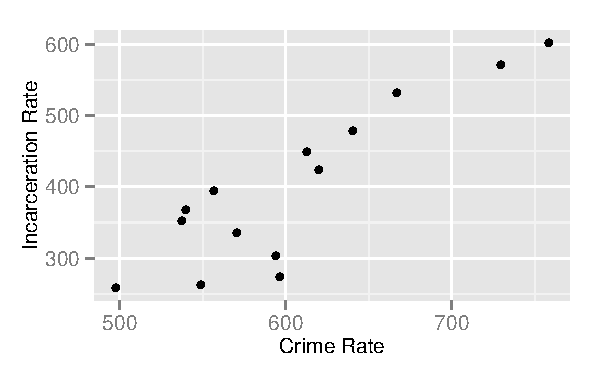
\includegraphics{figures/crime/crime_vs_incarceration_before_1991.pdf}
    \caption{1978--1991}\label{fig:before_1991}
  \end{figure}

  \begin{figure}[H]
    \centering
    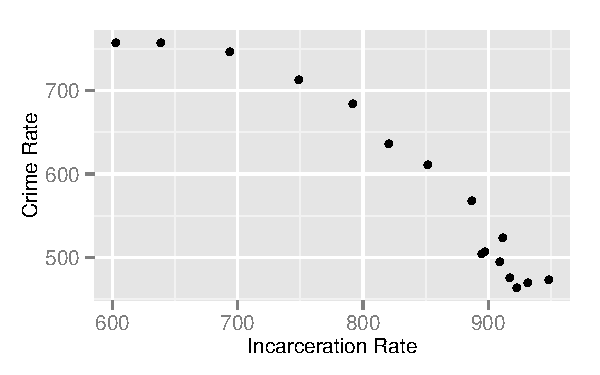
\includegraphics{figures/crime/incarceration_vs_crime_after_1991.pdf}
    \caption{1991--2006}\label{fig:after_1991}
  \end{figure}

  \begin{figure}[H]
    \centering
    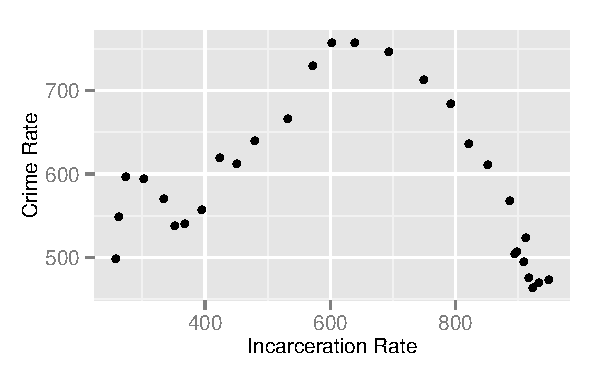
\includegraphics{figures/crime/incarceration_vs_crime.pdf}
    \caption{All Years}\label{fig:all_years}
  \end{figure}

  \begin{figure}[H]
    \centering
    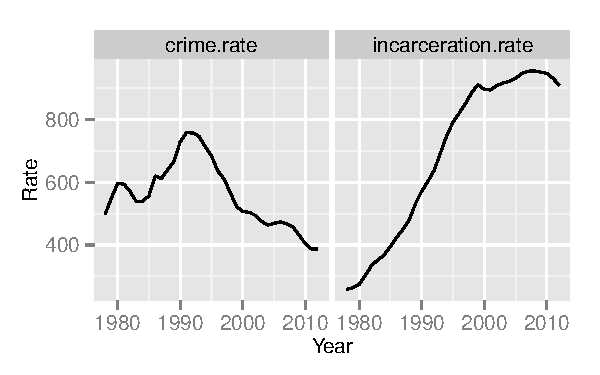
\includegraphics{figures/crime/rates_over_time.pdf}
    \caption{Rates over time}\label{fig:rates_over_time}
  \end{figure}
\end{document}

